\documentclass[../main.tex]{subfiles}




\begin{document}



\chapter{Homotopia}

\section{Homotopies entre aplicacions}

Denotem per $I$ l'interval tancat $[0,1]$ amb la topologia induïda per la recta real $\mathbb{R}$.

\begin{defi}
[Homotopia]\label{def:homotopia}\index{Homotopia}\index{Homotopia entre aplicacions} Siguin $X,Y$ dos espais topològics, i $f:X\rightarrow Y$, $g:X\rightarrow Y$ dues aplicacions contínues entre espais topològics. Una \textit{homotopia} de $f$ a $g$ és una aplicació contínua
\begin{equation}
    \notag
    H:X\times I \longrightarrow Y
\end{equation}
tal que $H(x,0) = f(x)$ i $H(x,1) = g(x)$, per a tot $x\in X$. Escriurem $f\simeq g$ si existeix alguna homotopia de $f$ a $g$. 
\end{defi}

\begin{defi}
[Homotopia relativa a un subconjunt]\label{def:homotopiarelativaaconjunt}\index{Homotopia relativa a un conjunt} Una homotopia entre dues aplicacions $f,g:X\rightarrow Y$ es diu \textit{relativa a} $A\subseteq X$ si $f(a) = g(a),\;\forall a\in A$.
\end{defi}

La idea essencial d'aquesta definició és que si jo tinc dues funcions $f:X\rightarrow Y$ i $g:X\rightarrow Y$, direm que $f\simeq g$ si es pot deformar $f$ de forma contínua fins a obtenir $g$. És a dir, es tracta de moure $f$ fent un ``desfaçament'' continu, fins a obtenir $g$. Després, si és una homotopia relativa a $A$, vol dir que es queden quiets els punts d'$A$ al efectuar aquest ``desfaçament''.

A continuació escriuré un seguit de proposicions i corol·laris que es corresponen a diferents exercicis proposats que, com són molt teòrics i poden servir per fer exercicis posteriorment, els he inclòs en forma de teoria. Ara, però, aquesta teoria no ha sigut donada pel professor.

\begin{prop}
[Exercici 1.1]\label{exercici1.1} Per a qualsevol parell d'espais topològics $X,Y$ la relació d'homotopia $f\simeq g$ és una relació d'equivalència en el conjunt de les aplicacions contínues $\{f:X\rightarrow Y\;:\;f\text{ és contínua}\}$ per cada parell d'espais topològics $X,Y$. Denotarem per $[X,Y]$ el conjunt de classes d'equivalència.
\end{prop}
\begin{proof}
Hem de provar que la relació $\simeq$ compleix que és reflexiva, simètrica i transitiva.
\begin{itemize}
    \item \underline{Reflexiva ($f\simeq f$)}? Sí, ja que és suficient considerar l'homotopia
    \begin{equation}
        \notag
        \begin{array}{rl}
            H:X\times I & \longrightarrow Y \\
            (x,t) & \longmapsto H(x,t) = f(x)
        \end{array}
    \end{equation}
    que és clarament contínua ja que ho és $f$ i que es verifica
    \begin{equation}
        \notag
        H(x,0) = f(x),\qquad H(x,1) = f(x).
    \end{equation}
    
    \item \underline{Simètrica ($f\simeq g \Rightarrow g\simeq f$)}? Sí, doncs si $H:X\times I\rightarrow Y$ és la homotopia de $f$ a $g$, és a dir, $f\simeq_H g$, podem prendre
    \begin{equation}
        \notag
        \overline{H}(x,t) = H(x,1-t),
    \end{equation}
    que verifica
    \begin{equation}
        \notag
        \overline{H}(x,0)=H(x,1) = g(x),\qquad \overline{H}(x,1) = H(x,0) = f(x),
    \end{equation}
    i per tant $g\simeq f$.
    
    \item \underline{Transitiva ($f\simeq_{H_1}g,\;g\simeq_{H_2}h\Rightarrow f\simeq h$)?} Sí, doncs podem definir, a partir de $H_1$ i $H_2$,
    \begin{equation}
        \notag
        H(x,t):=\left\{
        \begin{array}{ll}
            H_1(x,2t), & 0\leq t\leq 1/2,\\
            H_2(x,2t-1)& 1/2\leq t\leq 1.
        \end{array}
        \right.
    \end{equation}
    i aleshores $H$ verifica que es contínua i que
    \begin{equation}
        \notag
        H(x,0) =H_1(x,0)=f(x),\qquad H(x,1) = H_2(x,1) = h(x),
    \end{equation}
    i podem concloure $f\simeq_H g$.
\end{itemize}
\end{proof}

\begin{prop}
[Exercici 1.2.a]\label{exercici1.2.a} Si $f_0,f_1:X\rightarrow Y$ i $g_0,g_1:Y\rightarrow Z$ són aplicacions contínues tals que $f_0\simeq f_1$ i $g_0\simeq g_1$ llavors $g_0\circ f_0\simeq g_1\circ f_1$.
\end{prop}
\begin{proof}
Tenim
\begin{itemize}
    \item $f_0\simeq f_1\Longrightarrow \exists F:X\times I\rightarrow Y$ tq $F(x,0)=f_0(x)$ i $F(x,1) = f_1(x)$
    \item $g_0\simeq g_1\Longrightarrow \exists G:Y\times I\rightarrow Z$ tq $G(y,0) = g_1(y)$, i $G(y,1)=g_1(y)$.
\end{itemize}
Volem troba $H:X\times I\rightarrow Z$ tal que $H(z,0)=(g_0\circ f_0)(z)$ i $H(z,1) = (g_1\circ f_1)(z)$. Definim el producte de funcions següent:
\begin{equation}
    \notag
    F\times id:X\times I\rightarrow Y\times I,
\end{equation}
de manera que tenim el següent diagrama:
\begin{equation}
        \notag
        \xymatrix{
            X\times H\ar[d]_{F\times id} \ar[r]^{H} & Z \\
            Y\times I \ar[ur]_G
        }
    \end{equation}
    on $H$ és clarament contínua ja que $F\times id$ és contínua per ser producte de contínues, $G$ és contínua per hipòtesis i $H(x,t) = G(F(x,t),t)$ és, per tant, contínua per ser composició de contínues. Finalment,
    \begin{equation}
        \notag
        H(x,0) = G(F(x,0),0) = G(f_0(x),0) = g_0(f_0(x)) = (g_0\circ f_0)(x), 
    \end{equation}
    \begin{equation}
        \notag
        H(x,1) = G(F(x,1),1) = G(f_1(x),1) = g_1(f_1(x)) = (g_1\circ f_1)(x)
    \end{equation}
    com es volia veure.
\end{proof}

\begin{prop}
[Exercici 3a]\label{exercici1.3.a} Si $f_0,f_1:X\rightarrow Y$ i $g_0,g_1:A\rightarrow B$ són aplicacions contínues i tals que $f_0\simeq f_1$ i $g_0\simeq g_1$, llavors $f_0\times g_0\simeq f_1\times g_1$, on $f_i\times g_i$ denota l'aplicació $f_i\times g_i:X\times A \rightarrow Y\times B$, $(f_i\times g_i)(x,a) = (f_i(x),g_i(a))$.
\end{prop}
\begin{proof}
$f_0\simeq f_1$ vol dir que $\exists F:X\times I\rightarrow Y$ tal que $F(x,0) = f_0(x),\;\forall x\in X$ i $F(x,1) = f_1(x),\;\forall x\in X$. $g_0\simeq g_1$ vol dir que $\exists G:A\times I\rightarrow B$, tal que $G(a,0) =g_0(a),\;\forall a\in A$, i $G(a,1) = g_1(a),\;\forall a\in A$.

Definim
\begin{equation}
    \notag
    \begin{array}{rl}
        H:(X\times A)\times I & \longrightarrow Y\times B \\
        (x,a,t) & \longmapsto (F(x,t),G(a,t))
    \end{array}
\end{equation}
Aleshores, amb això
\begin{equation}
    \notag
    H(x,a,0) = (F(x,0),G(a,0)) = (f_0(x),g_0(a)) = (f_0\times g_0)(x,a),\qquad \forall x\in X,\;\forall a\in A.
\end{equation}
De la mateixa manera
\begin{equation}
    \notag
    H(x,a,1) = (F(x,1),G(a,1)) = (f_1(x),g_1(a)) = (f_1\times g_1)(x,a),\qquad \forall x\in X,\;\forall a\in A.
\end{equation}
i això tot junt implica que $f_0\times g_0\simeq f_1\times g_1$.
\end{proof}


\begin{coro}
[Exercici 3b]\label{exercici1.3.b} Si $X\simeq Y$ i $A\simeq B$, aleshores $X\times A\simeq Y\times B$.
\end{coro}
\begin{proof}
Si $X\simeq Y$ aleshores existeixen aplicacions contínues $f:X\rightarrow Y$ i $g:Y\rightarrow X$ tals que $f\circ g\simeq id_Y$ i $g\circ f\simeq id_X$. De la mateixa manera, si $A\simeq B$ aleshores existeixen aplicacions contínues $f':A\rightarrow B$ i $g':B\rightarrow A$ tals que $f'\circ g'\simeq id_B$ i $g'\circ f'\simeq id_A$. Així doncs, definim
\begin{equation}
    \notag
    \begin{array}{rl}
        h_1:X\times A & \longrightarrow Y\times B \\
        (x,a) & \longmapsto (f(x),f'(a))
    \end{array}
    \qquad 
    \begin{array}{rl}
        h_2:Y\times B & \longrightarrow X\times A \\
        (y,b) & \longmapsto (g(x),g'(a))
    \end{array}
\end{equation}
que clarament són contínues perquè son composicions i productes de contínues i a més satisfan
\begin{equation}
    \notag
    (h_1\circ h_2)(x,a) = h_1(g(x),g'(x)) = (f(g(x)),f'(g'(x))) \Rightarrow 
\end{equation}
\begin{equation}
    \notag
    \Rightarrow h_1\circ h_2 = (f\circ g)\times (f'\circ g')\simeq id_Y\times id_B \simeq id_{Y\times B}
\end{equation}
i, anàlogament,
\begin{equation}
    \notag
    h_2\circ h_1\simeq id_{X\times A}
\end{equation}
que implica que aleshores $X\times A\simeq Y\times B$ com volíem veure.
\end{proof}

\begin{coro}
[Exercici 6]\label{exercici1.6} Un espai $X$ és arc-connex si i només si totes les aplicacions $*\rightarrow X$ són homòtopes, on $*$ denota l'espai format per un únic punt. En altres paraules, $X$ és arc-connex si i només si $\text{card}[*,X]=1$.
\end{coro}
\begin{proof}
Si $X$ és arc-connex, considerem les aplicacions 
\begin{equation}
    \notag
    f,g:*\longrightarrow X
\end{equation}
Aleshores, $f(*) = x$ i $g(*) = y$. Com $X$ és arc-connex, existeix un camí $\alpha:I\rightarrow X$ (aplicació contínua tal que $\alpha(0) = x$ i $\alpha(1) = y$). Com $*\times I = I$, tenim l'homotopia 
\begin{equation}
    \notag
    \begin{array}{rl}
        H:*\times I & \longrightarrow X \\
        (*,t) & \longmapsto H(*,t) = \alpha(t) 
    \end{array}
\end{equation}
que és contínua i que satisfà
\begin{equation}
    \notag
    H(*,0) = \alpha(0) = x = f(*),\qquad H(*,1) = \alpha(1) = y = g(*).
\end{equation}
i per tant $f\simeq g$, com volíem veure.

Recíprocament, considerem dos punts $x,y\in X$, i suposem que les aplicacions $f,g:*\rightarrow X$, $f(*)=x$, $g(*)=y$ són homòtopes. Això vol dir que existeix una homotopia $H:*\times I\rightarrow X$ tal que $H(*,0) = x$, $H(*,1)=y$. Per tant, l'aplicació $\alpha:I\rightarrow X$ definida com $\alpha(t) = H(*,t)$ és una aplicació contínua que a més satisfà que $\alpha(0) = H(*,0) = x$ i $\alpha(1) = H(*,1) = y$ i per tant és un camí. Així doncs $X$ és arc-connex.
\end{proof}



\section{Equivalències homotòpiques}

\begin{defi}
[Equivalència homotòpica]\index{Equivalència homotòpica}\label{def:equivalenciahomotopica} Una aplicació contínua $f:X\rightarrow Y$ entre dos espais topològics és una \textit{equivalència homotòpica} si existeix una aplicació contínua $g:Y\rightarrow X$ tal que $g\circ f\simeq id_X$ i $f\circ g\simeq id_Y$.
\begin{equation}
    \notag
    g\circ f: X\overset{f}{\longrightarrow} Y \overset{g}{\longrightarrow} X;\qquad f\circ g: Y\overset{g}{\longrightarrow}X\overset{f}{\longrightarrow}
\end{equation}
\end{defi}

\begin{defi}
[Homotòpicament equivalents]\label{def:homotopicamentequivalents}\index{Homotòpicament equivalents} Direm que un espai $X$ és \textit{homotòpicament equivalent} a un espai $Y$ si existeix alguna equivalència homotòpica $X\rightarrow Y$ i ho denotarem per $X\simeq Y$\footnote{A vegades també direm que $X$ és \textit{del mateix tipus d'homotopia}\index{Tipus d'homotopia} que $Y$}.
\end{defi}

\begin{ej}\label{ej:dischomotopicamentequivalentapunt}
Sigui $D^2$ el disc tancat unitat de $\mathbb{R}^2$, és a dir, $D^2 = \{(x,y)\in \mathbb{R}^2\;:\;x^2+y^2\leq 1\}$. Sigui $p\in\mathbb{R}^2$ un punt qualsevol. Definim aleshores $X = D^2$ (amb la topologia induïda de $\mathbb{R}^2$) i $Y = \{p\}$. Veiem que $X\simeq Y$. 

Definim $f:X\rightarrow Y$ com $f(x,y)\in p$, $\forall (x,y)\in D^2$, i definim $g:Y\rightarrow X$ com $g(p) = (0,0)$. Aleshores $f$ és contínua ja que és una funció constant i $g$ també. A més,
\begin{equation}
    \notag
    (g\circ f)(x,y) = g(f(x,y)) = g(p) = (0,0),\qquad (f\circ g)(x,y) = f(g(x,y)) = f(0,0) = p
\end{equation}
cosa que implica que $g\circ f\equiv (0,0)$ i $f\circ g = id_Y$. 
\begin{equation}
    \notag
    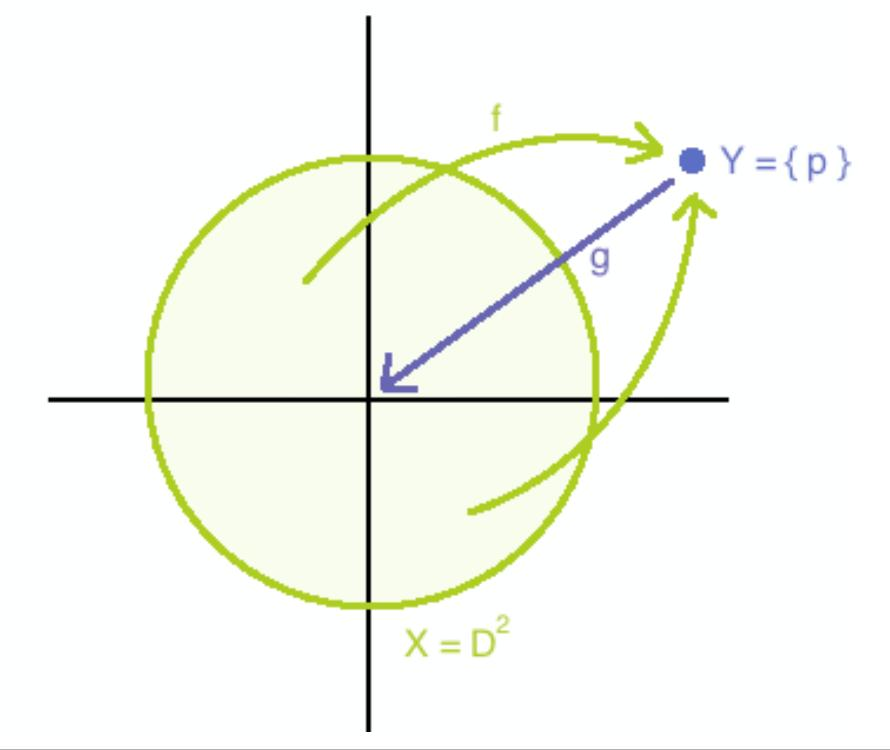
\includegraphics[scale = 0.2]{fotos_topo_2/fotos_mathonline/exemplepuntidischomotopicamentequivlents.jpeg}
\end{equation}
Aleshores, clarament $id_Y\simeq id_Y$ per la propietat reflexiva de la relació d'homotopia, per tant $f\circ g\simeq id_Y$. Queda veure que $g\circ f\simeq id_X$. Sigui $H:X\times I\rightarrow Y$ l'aplicació definida per $H(x,t) = (1-t)(x,t)$. Clarament $H$ és contínua i $H(x,0) = (x,y) = id_X(x,y)$, i $H(x,1) = (0,0) = (g\circ f)(x,y)$ i així $g\circ f\simeq id_X$ cosa que prova que $D^2\simeq \{p\}$.
\end{ej}

\begin{prop}
[Exercici 1.2.b]\label{exercici1.2.b} Aquesta relació és una relació d'equivalència entre espais topològics. 
\end{prop}
\begin{proof}
Com sempre, hem de provar les tres propietats. 

La propietat reflexiva és clara ja que si prenem $g=f=id$, es compleix $X\simeq X$.

La propietat simètrica és òbvia ja que la propia definició te la dona: $X\simeq Y \Longleftrightarrow \exists f:X\rightarrow Y$, $\exists g:Y\rightarrow X$ tq $f\circ g\simeq id$ i $g\circ f\simeq id$.

La propietat transitiva també es compleix. Suposem $X\simeq Y$ i $Y\simeq Z$. Aleshores existeixen aplicacions contínues
\begin{equation}
    \notag
    a:X\rightarrow Y,\quad b:Y\rightarrow X,\qquad c:Y\rightarrow Z,\quad d:Z\rightarrow Y
\end{equation}
tals que
\begin{equation}
    \notag
    a\circ b\simeq id_X,\quad b\circ a\simeq id_Y,\qquad c\circ d \simeq id_Y,\quad d\circ c\simeq id_Z.
\end{equation}
Aleshores, definint $f:=c\circ a:X\rightarrow Z$ i $g:=d\circ b:Z\rightarrow X$ obtenim dues funcions clarament contínues (composició de contínues és contínua) i que compleixen que
\begin{equation}
    \notag
    g\circ f = (d\circ b)\circ(c\circ a) = d\circ(b\circ c)\circ a \simeq d\circ c\circ a\circ b\simeq id
\end{equation}
on, en la primera relació $\simeq$ hem aplicat l'apartat (a, \ref{exercici1.2.a}) de l'exercici juntament amb la ja provada propietat de simetria d'aquesta relació. El mateix es fa per $f\circ g$.
\end{proof}

Per fer-nos una idea mental del que estem fent ho podem entendre de la següent manera: Un espai $X$ topològic és homotòpicament equivalent a un altre $Y$ si nosaltres podem anar deformant $X$ fins a obtenir $Y$ d'una forma contínua, és a dir, sense trencar l'espai ni enganxar coses. Per exemple, podríem dir el clàssic exemple que una tassa de cafè és homotòpicament equivalent a un tor, ja que nosaltres podem deformar el tor fins a obtenir la tassa de cafè (o a l'inrevés, ja que és d'equivalència) sense haver de trencar en cap moment el tor. Així com una esfera pot ser deformada en un sol punt sense trencar-la, però un tor no.

O sigui el que hem de fer és imaginar-nos que el nostre espai és de plastilina i que el podem anar mollejant, sempre i quan no li afegim forats, ni eliminem els que ja té ni trenquem la plastilina. No podem separar cap plastilina en cap moment, només donar-li forma.


\begin{prop}
\label{prop:propietatsequivalenciahomotopica}
\begin{enumerate}[(1)]
    \item Tot homeomorfisme és una equivalència homotòpica. Per tant, si dos espais $X$ i $Y$ són homeomorfs, llaors $X$ i $Y$ són homotòpicament equivalents.
    \item Les equivalències homotòpiques no són ni injectives ni exhaustives, en general.
\end{enumerate}
\end{prop}

\begin{prop}
[Exercici 11]\label{prop:aplicacionoexhaustivahomotopa}\label{exercici1.11} Si una aplicació contínua $f:X\rightarrow S^n$ no és exhaustiva, llavors és homòtopa a una aplicació constant.
\end{prop}
\begin{proof}
Si $f:X\rightarrow S^n$ no és exhaustiva, existeix un punt $x_0\in S^n$ tal que $x_0\not\in f(X)$. Per tant, $f$ factoritza així:
\begin{equation}
    \notag
    f:X\underset{g}{\longrightarrow} S^n\setminus \{x_0\}\underset{i}{\hookrightarrow} S^n.
\end{equation}
Ara bé, $S^n\setminus\{x_0\}\cong \mathbb{R}^n$ (per la projecció estereogràfica), i per tant, com $\mathbb{R}^n$ és estrellat, aleshores és contràctil, $\mathbb{R}^n\simeq *$ i per tant,
\begin{equation}
    \notag
    f:X\underset{g}{\rightarrow}S^n\setminus\{x_0\}\simeq *\underset{i}{\hookrightarrow}S^n.
\end{equation}
O sigui que $f=i\circ g\simeq i\circ\varepsilon_a=\varepsilon_a$.
En definitiva, $f$ és homòtopa a una aplicació constant.
\end{proof}


\section{Espais contràctils}

\begin{defi}
[Contràctil]\index{Contràctil}\label{def:contractil} Denotem per $*$ l'espai que només conté un element. Un espai $X$ tal que $X\simeq *$ es diu \textit{contràctil}.
\end{defi}

Seguint la nostra manera intuïtiva de veure això, un espai contràctil és doncs un espai que pot ser deformat en un sol punt. Per exemple, una esfera pot ser contràctil ja que pot ser aixafada i comprimida en un sol punt. Però un tor no ho és, ja que per ser aixafat en un sol punt, ens hauríem de menjar el seu forat i aleshores la deformació no és contínua.

\begin{prop}[Exercici 8]\label{exercici1.8}
\label{prop:propietatscontractil} Un espai $X$ és contràctil si i només si l'aplicació identitat $id_X:X\rightarrow X$ és homòtopa a una aplicació constant\footnote{Una aplicació $c:X\rightarrow Y$ es diu \textit{constant}\index{Aplicació constant} si existeix algun element $q\in Y$ tal que $c(x) = q$ per a tot $x\in X$.}.
\end{prop}
\begin{proof}
Suposem que $X$ és contràctil. Per definició, es té doncs, $X\simeq *$. O sigui que existeixen aplicacions
\begin{equation}
    \notag
    f:X\rightarrow *,\quad g:*\rightarrow X,\quad \text{tq.}\left\{
    \begin{array}{ll}
        g\circ f\simeq id_X,\\
        f\circ g\simeq id_*
    \end{array}
    \right.
\end{equation}
Notem que $x_0 = g(*)$. Aleshores, la primera homotopia $g\circ f\simeq id_X$ ens diu que la identitat de $X$ és homòtopa a $g\circ f (x) = g(*)=x_0$. O sigui que la identitat de $X$ és homòtopa a l'aplicació constant $\varepsilon_{x_0}(x) = x_0$ (aquesta és una notació per expressar l'aplicació constant que sempre dona $x_0$).

Recíprocament, si $id_X\simeq \varepsilon_{x_0}$, podem considerar les aplicacions
\begin{equation}
    \notag
    f:X\rightarrow *,\;f(x) = *,\qquad g:*\rightarrow X,\;g(*)=x_0
\end{equation}
i és immediat que $f\circ g = id_*$ mentre que $g\circ f(x) = \varepsilon_{x_0}(x)$. Com que per hipòtesi, $\varepsilon_{x_0}\simeq id_X$, tindrem
\begin{equation}
    \notag
    g\circ f = \varepsilon_{x_0}\simeq id_X,\qquad f\circ g\simeq id_*
\end{equation}
o sigui $X\simeq *$.
\end{proof}

\begin{prop}[Exercici 5]\label{exercici1.5}
\label{prop:propietatshomotopiques} La connexió i l'arc-connexió són \textit{propietats homotòpiques}\footnote{Una \textit{propietat homotòpica}\index{Propietat homotòpica} és una propietat d'un espai topològic $X$ que satisfà que si $X\simeq Y$, aleshores $Y$ també té aquesta propietat.}. Però la compacitat i les propietats de separació no són propietats homotòpiques.
\end{prop}
\begin{proof}
Suposem que $X$ és connex, que $X\simeq Y$, però $Y$ no és connex. Recordem que això vol dir que aleshores $\exists U,V\subseteq Y$ tals que $Y = U\cup V$ amb $U,V\not=\emptyset$ i $U\cap V\not=\emptyset$. Ara, per definició, $X\simeq Y$ si existeixen aplicacions $f:X\rightarrow Y$ i $g:Y\rightarrow X$ tals que $g\circ f \simeq id_X$ i $f\circ g\simeq id_Y$, on $f\circ g\simeq id_Y$ volia dir que $\exists H:Y\times I\rightarrow Y$ amb $H(y,0) = f(g(y))$ i $H(y,1) = id_Y(y) = y$, $\forall y\in Y$. Ara, de Topologia, sabem que si $f:X\rightarrow Y$ és una aplicació contínua i $X$ és connex, aleshores $f(X)$ és connex. Aleshores, 
\begin{equation}
    \notag
    f(X) = (f(X)\cap U)\cup (f(X) \cap V)
\end{equation}
on $f(X)\cap U$ i $f(X)\cap V$ són dos oberts de $f(X)$, que és connex. Però $U\cap V = \emptyset$ i $f(X)$ és obert. Per tant algun dels dos ha de ser $\emptyset$. Posem $f(X)\cap V = \emptyset$. Aleshores $f(X)\subseteq U$ i llavors tenim
\begin{equation}
    \notag
    H(y,0) = f(g(y))\in U,\qquad H(y,1) = y\in V
\end{equation}
Però $\{y\}\times I$ és un subespai connex de $Y\times I$ i pel mateix raonament d'abans, o bé $H(\{y\}\times I)\subseteq U\times I$, o bé $H(\{y\}\times I)\subseteq V\times I$. En qualsevol dels dos casos arribem a una contradicció. Per tant, $Y$ és connex com volíem veure.

Com que connex implica arc-connex, automàticament obtenim que $Y$ és arc-connex i per tant l'arc-connexió és una propietat homotòpica.

Finalment, veiem que si $X$ és de Hausdorff i $X\simeq Y$, aleshores $Y$ no té per què ser de Hausdorff. Veiem un  contraexemple: prenem $X = \{0\}\subseteq \mathbb{R}$ amb la topologia grollera\footnote{Recordem que la topologia grollera era la que tenia com a únics oberts els conjunts $\emptyset$ i $X$\index{Topologia grollera}.}. Aleshores $X$ és de Hausdorff. Prenem $Y = \{p,q\}\subseteq\mathbb{R}$ amb la topologia grollera. Llavors $Y$ no és de Hausdorff. Definim les aplicacions
\begin{equation}
    \notag
    f:X\rightarrow Y,\qquad g:Y\rightarrow X
\end{equation}
com $f(0) = p$ i $g(p) = g(q) = 0$. Aquestes són aplicacions contínues que a més satisfan que $g\circ f\simeq id$ i $f\circ g\simeq id$. Veiem això últim. Definim l'aplicació
\begin{equation}
    \notag
    H:Y\times I\rightarrow Y,\qquad H(y,t) := \left\{
    \begin{array}{rcl}
        y & \text{si} & t\leq 1/2 \\
        p & \text{si} & t\geq 1/2
    \end{array}
    \right.
\end{equation}
que és contínua clarament ja que $Y$ té la topologia grollera i se satisfà $H(y,0) = x = f(g(y)) = id(y)$, $\forall y\in Y$ i $H(y,1) = p = g(f(x))$, $\forall x\in X$, cosa que implica que $X\simeq Y$. Per tant, hem trobat un contraexemple que il·lustra que la propietat de Hausdorff no és homotòpica. El mateix es pot fer per la resta de propietats de separació.
\end{proof}

\begin{defi}
[Estrellat]\index{Subconjunt estrellat}\index{Estrellat}\label{def:estrellat} Un subconjunt $X$ de $\mathbb{R}^n$ s'anomena estrellat si existeix un punt $x_0\in X$ tal que el segment que uneix $x_0$ amb qualsevol altre punt de $X$ és contingut a $X$.
\end{defi}

En altres paraules, $X$ s'anomena estrellat si $\exists x_0\in X$ centre tal que $\forall x\in X$, es compleix
\begin{equation}
    \notag
    \{(1-t)x_0 +tx\}_{0\leq t\leq 1}\subseteq X
\end{equation}

\begin{prop}
[Exercici 7]\label{exercici1.7}
\begin{enumerate}[(a)]
    \item Tot subconjunt convex de $\mathbb{R}^n$ és estrellat.
    \item Tot subconjunt estrellat de $\mathbb{R}^n$ és contràctil.
\end{enumerate}
\end{prop}
\begin{proof}
\begin{enumerate}[(a)]
    \item Ni idea
    \item Volem provar que $X$ és contràctil, és a dir, que tota parella d'aplicacions $f:X\rightarrow *$ i $g:*\rightarrow X$ satisfà $f\circ g\simeq id_*$ i $g\circ f\simeq id_X$. La primera és clara, ja que la composició dona la identitat. Anem a veure que $f\circ g\simeq id_X$. Definim
    \begin{equation}
        \notag
        \begin{array}{rl}
            H:X\times I & \longrightarrow X \\
            (x,t) & \longmapsto H(x,t):=(1-t)x_0+tx
        \end{array}
    \end{equation}
    Clarament és una funció contínua ja que és polinòmica. A més, satisfà que
    \begin{equation}
        \notag
        \left.
        \begin{array}{ll}
            H(x,0) = x_0 = \varepsilon_{x_0}(x) \\
            H(x,1) = x = id_X(x)
        \end{array}
        \right\} \Longrightarrow id_X\simeq \varepsilon_{x_0}
    \end{equation}
    on $\varepsilon_{x_0}$ simbolitza la funció constant igual a $x_0$. Aleshores,
    \begin{equation}
        \notag
        (g\circ f)(x) = g(f(x))= g(*) = x_0\Longrightarrow g\circ f= \varepsilon_{x_0}
    \end{equation}
    i així obtenim $g\circ f\simeq id_X$. Per tant $H$ és una homotopia i ens dona que $X\simeq *$, com volíem veure.
\end{enumerate}
\end{proof}

\begin{ej}
[Exercici 9]\label{exercici1.9} Si $X\not=\emptyset$, l'espai $CX=(X\times [0,1])/(X\times \{1\})$ és contràctil.
\end{ej}


\subsection{Retractes}

\begin{defi}
[Retracció]\index{Retracció}\label{def:retraccio} Sigui $X$ un espai topològic i sigui $A\subseteq X$ un subespai. Denotem per $i:A\rightarrow X$ la inclusió. Una aplicació contínua $r:X\rightarrow A$ tal que $r\circ i = id_A$ s'anomena una \textit{retracció} de $X$ en $A$. Llavors també diem que $A$ és un \textit{retracte} de $X$.\index{Retracte}
\end{defi}

Intuïtivament, un subespai $A$ és un retracte de $X$ si $X$ pot ser contínuament deformat per convertir-se en $A$, fixant tots els punts d'$A$. Un gràfic orientatiu seria el següent:
\begin{equation}
    \notag
    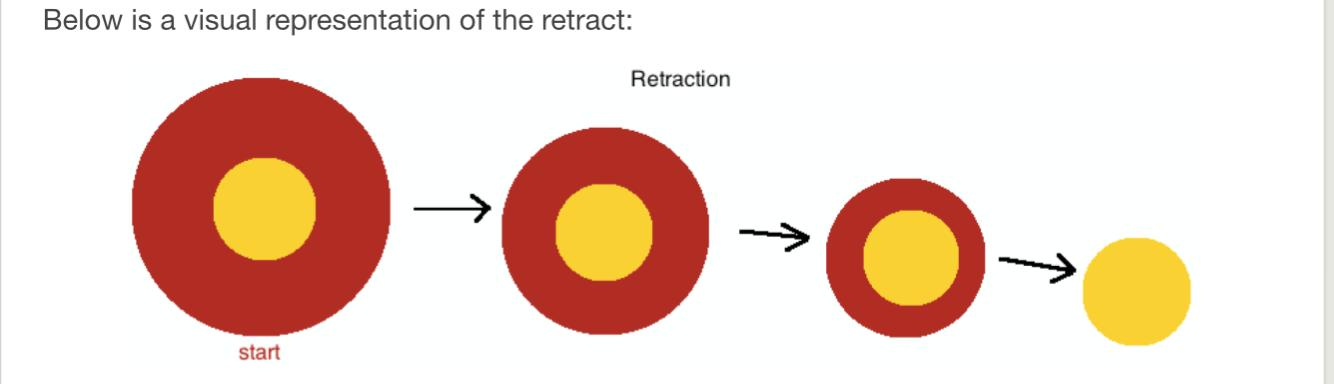
\includegraphics[scale = 0.25]{fotos_topo_2/fotos_mathonline/retraccio.jpeg}
\end{equation}

\begin{ej}
\label{ej:retraccio} Sigui $D^2$ el disc unitat tancat en $\mathbb{R}^2$. Sigui $\frac{1}{2}D^2$ el disc tancat amb radi $1/2$ i centre a l'origen. Veurem que $\frac{1}{2}D^2$ és un retracte de $D$. 

Definim una retracció $r:X\rightarrow A$ per $r(x,y) = (a,b)$, on $(a,b)$ satisfà que 
\begin{equation}
    \notag
    d((x,y),(a,b)) = \inf_{(c,d)\in \frac{1}{2}D^2}d((x,y),(c,d)).
\end{equation}
En altres paraules, cada punt $(x,y)\in D^2$ té la seva imatge igual a un punt $(a,b)\in \frac{1}{2}D^2$ la distància del qual des de $(x,y)$ és minimitzada. Clarament $r$ és una aplicació contínua. A més, $r\circ i = id_A$. Aleshores, de fet, $\frac{1}{2}D^2$ és un retracte de $D^2$.
\begin{equation}
    \notag
    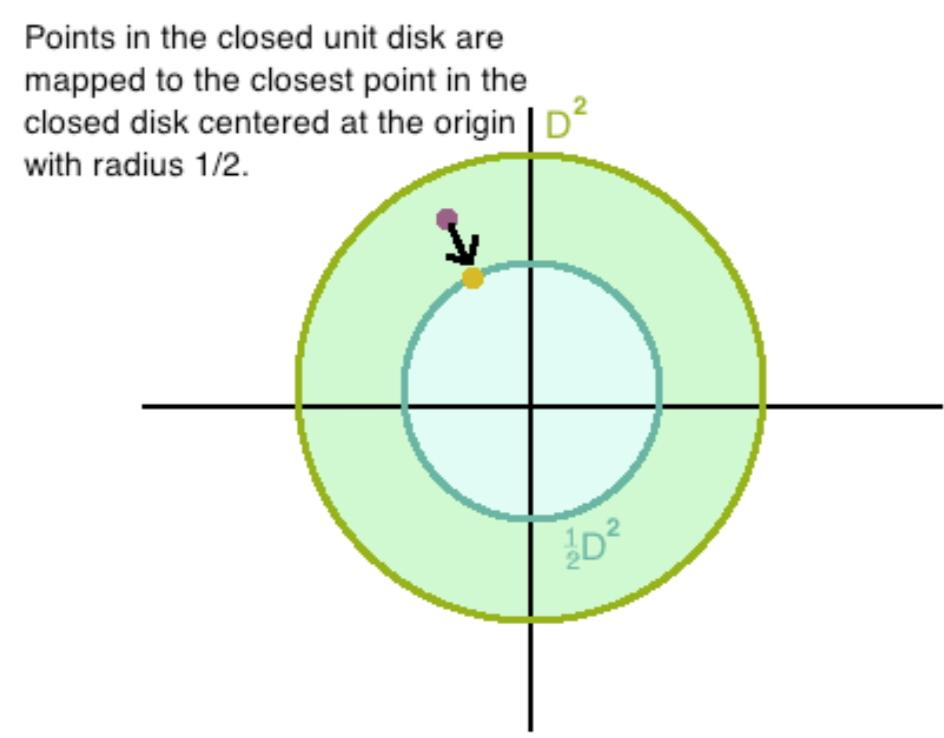
\includegraphics[scale = 0.25]{fotos_topo_2/fotos_mathonline/retracte.jpeg}
\end{equation}
\end{ej}

\begin{prop}
\label{prop:propietatretracte1} Qualsevol punt d'un espai $X$ és un retracte de $X$.
\end{prop}
\begin{proof}
Considerem la funció $r:X\rightarrow \{a\}$, definida per tota $x\in X$ per $r(x) = b$. Aleshores, $r$ és, trivialment una funció contínua. A més a més, prenent l'aplicació inclusió $i:\{a\}\rightarrow X$, tenim $r\circ i (a) = a$, per tant $r\circ i = id_{\{a\}}$, per tant $\{a\}$ és un retracte de $X$.
\end{proof}

\begin{prop}
[Exercici 10]\label{prop:rectractecontractil}\label{exercici1.10} Tot retracte d'un espai contràctil és contràctil.
\end{prop}
\begin{proof}
Suposem que $X$ és contràctil i que $A\subseteq X$ és un retracte de $X$. Així, existeix una aplicació contínua
\begin{equation}
    \notag
    r:X\rightarrow A,\quad r(x)=x,\;\forall x\in A
\end{equation}
que li diem retracció. Utilitzarem la caracterització dels espais contràctils de l'exercici 8 (\ref{exercici1.8}), que deia que $A$ és contràctil sii $1_A\simeq \varepsilon_{a_0}$ (on $\varepsilon_{a_0}(y) = a_0,\forall y\in A$).

Com $X$ és contràctil, $1_X\simeq \varepsilon_{x_0}$. Si denotem $i:A\hookrightarrow X$ la inclusió, la igualtat $r(x) = x$, $\forall x\in A$, s'expressa $r\circ i = 1_A$. Aleshores,
\begin{equation}
    \notag
    1_A=r\circ i=r\circ 1_X\circ i\simeq r\circ\varepsilon_{x_0}\circ i=\varepsilon_{r(x_0)}.
\end{equation}
Per tant $A$ és contràctil.
\end{proof}

\subsection{Deformacions}

\begin{defi}
[Deformació]\label{def:deformacio}\index{Deformació} Una retracció $r:X\rightarrow A$ s'anomena \textit{deformació} de $X$ en $A$ si $i\circ r\simeq id_X$. Un subespai $A$ és un \textit{retracte de deformació}\index{Retracte de deformació} de $X$ si existeix una deformació de $X$ en $A$.
\end{defi}

Veiem un exemple per veure quina és la idea d'aquesta definició.

\begin{ej}
\label{ej:deformacio}
Considerem l'espai $A = S^1$ que és el cercle unitat i $X = S^1\times I$ que és el cilindre unitat. $A$ és un retracte de deformació de $X$:
\begin{equation}
    \notag
    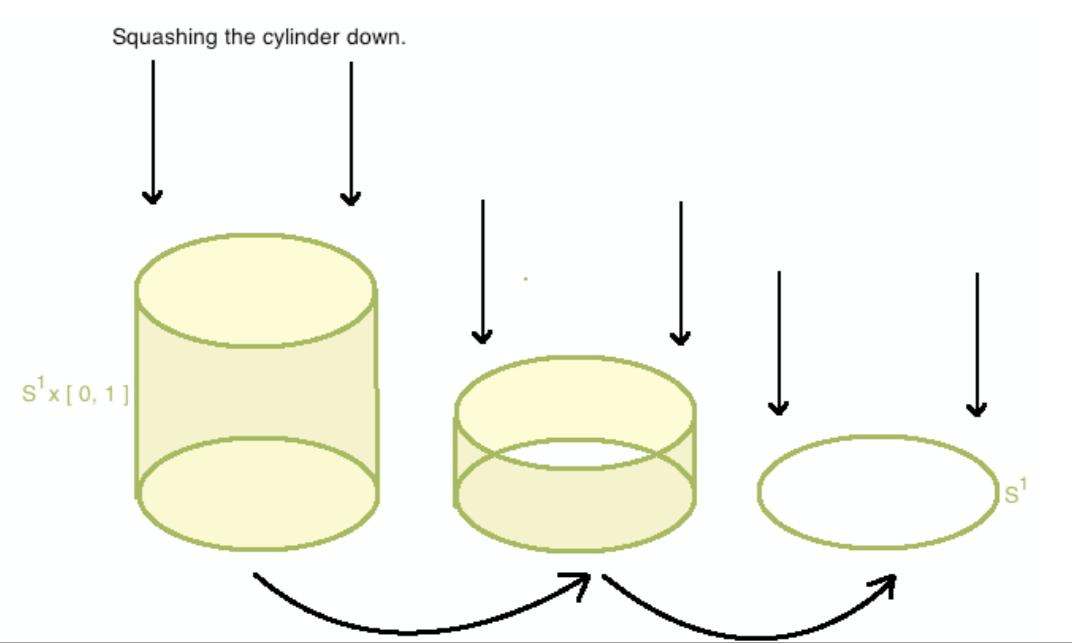
\includegraphics[scale = 0.25]{fotos_topo_2/fotos_mathonline/deformacio.jpeg}
\end{equation}
\end{ej}

\begin{prop}
Si $A$ és un retracte de deformació de $X$, llavors $A\simeq X$.
\end{prop}

\begin{prop}
Un espai $X$ és contràctil si i només si qualsevol dels seus punts és un retracte de deformació de $X$.
\end{prop}

\begin{prop}
Tot retracte d'un espai de Hausdorff és un subespai tancat.
\end{prop}

\begin{exercici}
[Exercici 14]\label{exercici1.14} Demostreu que cadascun dels espais següents és homotòpicament equivalent a una unió puntual d'una o més esferes i determineu la dimensió d'aquestes esferes en cada cas:
\begin{enumerate}[(a)]
    \item $\mathbb{R}^n\setminus\{p_1,\ldots,p_k\}$, on $p_i\not=p_j$, per $i\not=j,\;i,j=1,\ldots,k$.
    \item $\mathbb{R}^n\setminus \mathbb{R}^m$, on $m\leq n-2$.
    \item $\mathbb{R}^3$ menys $n$ rectes concurrents.
\end{enumerate}
\end{exercici}
\begin{sol}
\begin{enumerate}[(a)]
    \item Per simplificar aquest problema, utilitzarem un resultat que afirma que donats uns punts de $\mathbb{R}^n$, $p_1,\ldots,p_k$, existeix un homeomorfisme $\mathbb{R}^n\setminus \{p_1,\ldots,p_k\}\cong \mathbb{R}^n\setminus \{q_1,\ldots,q_k\}$, essent $q_i = (2i-1,0,\ldots,0)$. De forma que podem fer el problema buscant els $q_i$, que és més fàcil.
    
    Aleshores, l'homotopia que busquem és la que s'expressa com la retracció de $\mathbb{R}^n\setminus\{q_1,\ldots, q_k\}$ sobre les esferes de radi 1 i centre aquests punts. Gràficament és
    \begin{equation}
        \notag
        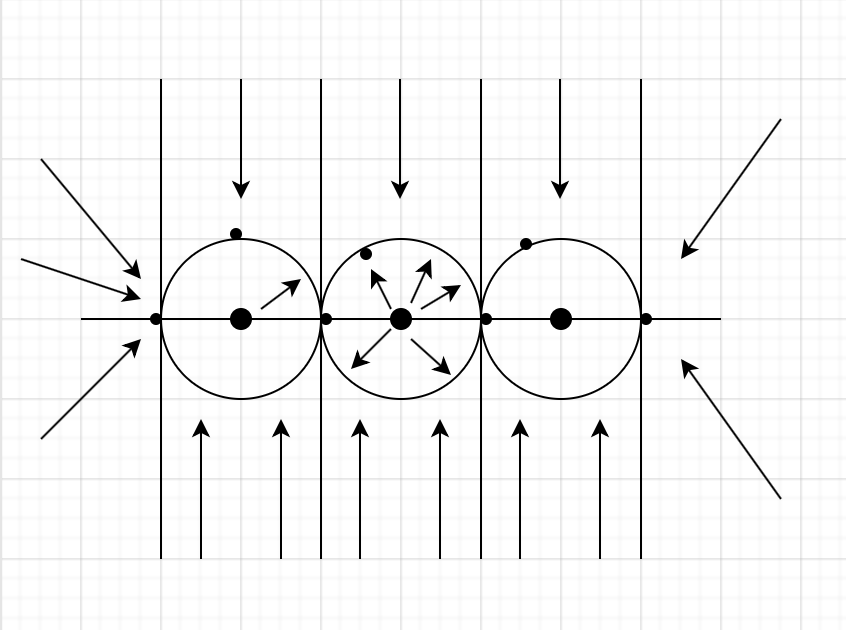
\includegraphics[scale = 0.5]{fotos_topo_2/otrasfotos/uniopuntualesferes.png}
    \end{equation}
    Això és,
    \begin{itemize}
        \item dins de cada esfera és la projecció radial des del centre de l'esfera sobre l'esfera.
        \item entre $q_1-1$ i $q_k+1$ és la projecció vertical sobre l'esfera,
        \item fins $q_1-1$ és la projecció radial a $(q_1-1,0,\ldots,0)$,
        \item a partir de $q_k+1$ és la projecció radial a $(q_k+1,0,\ldots,0)$.
    \end{itemize}
    En definitiva,
    \begin{equation}
        \notag
        \mathbb{R}^n\setminus\{p_1,\ldots,p_k\}\simeq S_{q_1}^{n-1}\vee S_{q_2}^{n-1}\vee\cdots\vee S_{q_k}^{n-1}.
    \end{equation}
    
    \item $\mathbb{R}^n\setminus\mathbb{R}^m=\mathbb{R}^m\times(\mathbb{R}^{n-m}\setminus \{0\})$. Com $\mathbb{R}^n-m\setminus\{0\}\simeq S^{n-m-1}$ (per la projecció radial, l'esfera és un retracte de deformació fort de $\mathbb{R}^{n-m}\setminus\{0\}$) tindrem
    \begin{equation}
        \notag
        \mathbb{R}^n\setminus\mathbb{R}^m\simeq \mathbb{R}^m\times S^{n-m-1}
    \end{equation}
    i com $\mathbb{R}^m$ és contràctil (ja que és convex), tenim $\mathbb{R}^m\simeq *$. En definitiva:
    \begin{equation}
        \notag
        \mathbb{R}^n\setminus \mathbb{R}^m\simeq *\times S^{n-m-1}=S^{n-m-1}.
    \end{equation}
    
    \item Considerem que el punt de concurrència de les $n$ rectes és el origen $O$. Aleshores, per projecció radial des de l'origen
    \begin{equation}
        \notag
        \mathbb{R}^3\setminus\{\ell_1,\ldots,\ell_n\}\simeq S^2\setminus\{p_{\pm1},\ldots,p_{\pm n}\}
    \end{equation}
    on $\ell_1,\ldots,\ell_n$ són les rectes concurrents en l'origen, i $p_{\pm i} = S^2\cap \ell_i$.
    
    Ara, com $S^2\setminus\{\text{punt}\}\cong \mathbb{R}^2$, es té que 
    \begin{equation}
        \notag
        S^2\setminus\{2n\text{ punts}\}\cong \mathbb{R}^2\setminus\{2n-1\text{ punts}\}
    \end{equation}
    i, aplicant l'apartat (a), es té que finalment 
    \begin{equation}
        \notag
        \mathbb{R}^3\setminus\{\ell_1,\ldots,\ell_n\;:\;\bigcap_{i=1}^n \ell_i = O\}\simeq S_{q_1}^2\vee S_{q_2}^2\vee\cdots\vee S_{q_{2n-1}}^2.
    \end{equation}
\end{enumerate}
\end{sol}







\section{Homotopia de camins}

\begin{defi}
[Homotopia relativa]\label{def:homotopiarelativa}\index{Homotopia relativa} Sigui $A$ un subespai d'un espai topològic $X$. Siguin $f_0:X\rightarrow Y$ i $f_1:X\rightarrow Y$ dues aplicacions contínues tals que $f_0(a)=f_1(a)$ per a tot punt $a\in A$. Una \textit{homotopia de $f_0$ a $f_1$ relativa a $A$} és una aplicació contínua $H:X\times I\rightarrow Y$ tal que $H(x,0) = f_0(x)$ i $H(x,1) = f_1(x)$ per a tot $x\in X$ i, a més, $H(a,t) = f_0(a)$ per a tot $a\in A$. Direm que $H$ és \textit{estacionària}\index{Estacionària}\index{Homotopia estacionària} en els punts de $A$.
\end{defi}

Recordem ara el que era un camí. Això és de Topologia. Un \textit{camí}\index{Camí} en un espai topològic $Y$ és una aplicació contínua $\alpha:I\rightarrow Y$. Si $x,y\in Y$, diem que $\alpha$ és un camí de $x$ fins a $y$ si se satisfà que $\alpha(0)= x$ i $\alpha(1) = y$. Direm que el camí és \textit{tancat}\index{Camí tancat} si $\alpha(0) = \alpha(1)$.

Així doncs, podem veure que tota homotopia $H:X\times I\longrightarrow Y$ defineix una família de camins $\{H_x\}_{x\in X}$, on $H_x(t) = H(x,t)$. Amb això observem també que l'homotopia $H$ és relativa a $A$ si $H_a$ és un camí constant per a tot $a\in A$.

Denotarem el fet que existeixi una homotopia de $f_0$ a $f_1$ relativa a un subespai $A$ per $f_0\simeq_A f_1$ o bé $f_0\simeq f_1$ rel $A$.

\begin{defi}
[Espai amb punt base]\label{def:espaiambpuntbase}\index{Espai amb punt base} Un \textit{espai amb punt base} és un parell $(X,p)$ on $X$ és un espai topològic i $p$ és un punt de $X$. Si $(X,p)$ i $(Y,q)$ són espais amb punt base, direm que una aplicació contínua $f:X\rightarrow Y$ \textit{conserva el punt base} si $f(p) = q$. Denotarem per $[(X,p),(Y,q)]$ el conjunt de classes d'equivalència d'aplicacions contínues $f:X\rightarrow Y$ amb $f(p)=q$ respecte a la relació d'homotopia relativa al subespai $\{p\}\subseteq X$.
\end{defi}

\begin{defi}
[Camins homòtops]\label{def:homotopiadecamins}\index{Homotopia de camins}\index{Camins homòtops} Dos camins $\sigma:I\rightarrow X$ i $\sigma':I\rightarrow X$ amb $\sigma(0) = \sigma'(0)$ i $\sigma(1)=\sigma'(1)$ es diuen \textit{homòtops relativament als extrems} si $\sigma\simeq \sigma'$ rel $\{0,1\}$. Així doncs, són homòtops relativament als extrems si existix una aplicació contínua $H:I\times I\rightarrow Y$ tal que $H(s,0)=\sigma(s)$ i $H(s,1) = \sigma'(s)$, per a tot $s\in I$ i, a més, $H(0,t) = p$ i $H(1,t) = q$ per a tot $t\in I$, on $p$ és l'origen comú de $\sigma$ i $\sigma'$ i $q$ el final comú.
\end{defi}

Per tal de simplificar la notació, habitualment es diu només que $\sigma$ i $\sigma'$ són \textit{homòtops}\index{Camins homòtops} o \textit{equivalents}\index{Camins equivalents} i s'escriu $\sigma\simeq\sigma'$ sense especificar que l'homotopia és relativa als extrems. De fet, si no imposéssim que les homotopies fossin relatives als extrems, llavors tots els camins serien homòtops a camins constants, ja que $I$ és contràctil.

Intuïtivament, podem entendre que dos camins són homòtops si podem deformar contínuament l'un en l'altre. Aquesta deformació contínua representa que és la funció homotopia $H$, que deforma un camí, a través del temps $t$, de forma contínua fins a obtenir l'altre. Amb forma contínua em refereixo a que no pot trencar el camí en cap moment, ni ajuntar els extrems ni fer res d'això.

Ara bé, la definició diu que són homòtops relativament a $\{0,1\}$. Això què vol dir? Doncs vol dir que els punts $\{0,1\}$ no es mouran al fer aquesta deformació. I aquests punts corresponen, per la definició de camí, al començament i al final dels camins. És a dir, si jo tinc dos camins $\sigma:I\rightarrow X$ i $\tau:I\rightarrow X$ tals que $\sigma(0) = \tau(0)=p$, i $\sigma(1) = \tau(1) = q$, aleshores, si $\sigma\simeq \tau$ es diuen que són homòtops relativament als extrems. Gràficament,
\begin{equation}
    \notag
    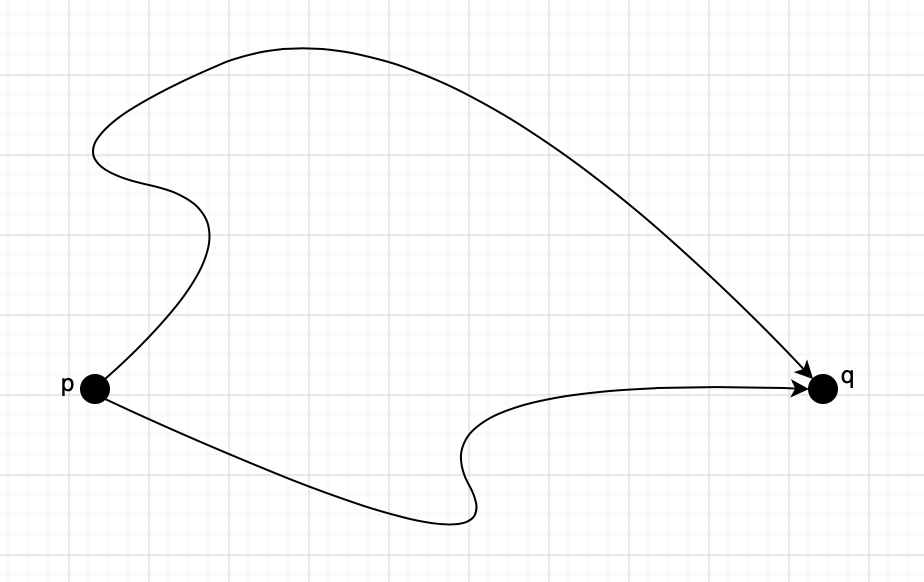
\includegraphics[scale = 0.5]{fotos_topo_2/otrasfotos/caminos.png}
\end{equation}
aquests són dos camins homòtops relativament als extrems ja que comparteixen els extrems i a més podem deformar un per obtenir l'altre de forma contínua, és a dir, sense trencar-lo ni afegir-hi res.

Vegem un exemple. Imaginem-nos que tenim una esfera $S^2$ i tenim un llaç (veure \ref{def:llaç}), que és només un camí tancat. Aleshores podem imaginar-nos aquest llaç com una goma de cabell. Aleshores tots els llaços que podem fer amb la goma a sobre de l'esfera seran camins homòtops. Així doncs, qualsevol llaç sobre $S^2$ serà homòtop a qualsevol altre, sempre i quan doni el mateix nombre de voltes.

Ara bé, què passa si en lloc d'una esfera tenim un tor. Aleshores podem prendre un llaç $\sigma$ que sigui la volt exterior del tor, i un altre llaç $\tau$ que envolti el tor passant pel forat. És a dir, gràficament:
\begin{equation}
    \notag
    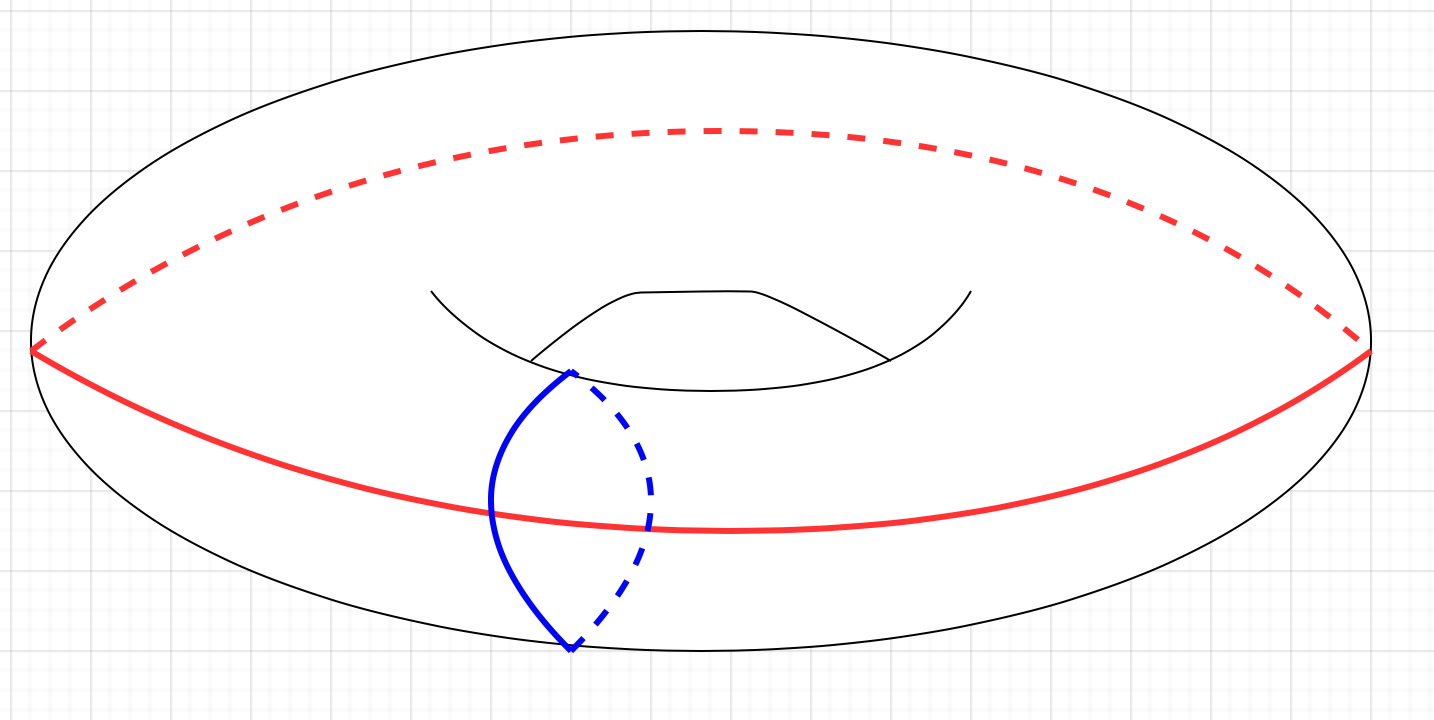
\includegraphics[scale = 0.5]{fotos_topo_2/otrasfotos/toroconcaminos.png}
\end{equation}
Aquí els camins vermell i blau no són homòtops, ja que per transformar l'un en l'altre caldria trencar-lo i després tornar-lo a enganxar.

\begin{nota}
Cal destacar que, generalment, si tenim dos camins $\alpha_1$ i $\alpha_2$ tals que $\alpha_1\simeq \alpha_2$, la notació $\alpha_1\simeq\alpha_2$ vol dir en realitat que existeix una homotopia entre els camins $\alpha_1$ i $\alpha_2$ relativa als extrems de l'interval $I=[0,1]$ encara que no es digui. És a dir, que existeix una aplicació contínua $H:I\times I\rightarrow X$ tal que $H(s,0)=\alpha_1(s)$, $H(s,1) = \alpha_2(s)$ i, a més, $H(0,t)= \alpha_1(0) = \alpha_2(0),\;\forall t\in I$, i $H(1,t) = \alpha_1(1)=\alpha_2(1)$ per a tot $t\in I$. Canviant la notació estem dient que $H_0 = \alpha_1$, $H_1 =\alpha_2$ i, a més, es compleix que $H_t(0) = \alpha_1(0)=\alpha_2(0)$ i $H_t(1) = \alpha_1(1)=\alpha_2(1)$, per tot $t\in I$.
\end{nota}

\begin{defi}
[Composició de camins]\label{def:composiciocamins}\index{Composició de camins} Si $\sigma:I\rightarrow X$ i $\omega:I\rightarrow X$ són dos camins a $X$ tals que $\sigma(1) = \omega(0)$, definim la \textit{composició} o el \textit{producte de camins}\index{Producte de camins} com el camí a $X$ donat per
\begin{equation}
    \notag
    (\sigma * \omega)(t) = \left\{
    \begin{array}{rl}
        \sigma(2t) & \text{si}\;0\leq t\leq\frac{1}{2},\\
        \omega(2t-1) & \text{si}\;\frac{1}{2}\leq t\leq 1.
    \end{array}
    \right.
\end{equation}
\end{defi}

Aquesta operació amb camins és compatible amb la relació d'homotopia; és a dir, si $\sigma\simeq\sigma'$ rel $\{0,1\}$ i $\omega\simeq\omega'$ rel $\{0,1\}$, llavors $\sigma*\omega\simeq \sigma'*\omega'$ rel $\{0,1\}$. Per tant, si denotem per $[\sigma]$ la classe d'homotopia del camí $\sigma$ i per $[\omega]$ la classe d'homotopia del camí $\omega$ (relativament als extrems), llavors l'operació $[\sigma]\cdotp [\omega]=[\sigma*\omega]$ està ben definida: no depèn dels representants escollits en cada classe.


\begin{prop}
[Exercici 2, llista 2]\label{exercici2.2} Si $\alpha_1,\alpha_2,\beta_1,\beta_2$ són camins en un espai $X$ amb $\alpha_1*\beta_1\simeq\alpha_2*\beta_2$ i a més $\alpha_1\simeq \alpha_2$, aleshores $\beta_1\simeq \beta_2$.
\end{prop}
\begin{proof}
Denotem $p = \alpha_1(0) = \alpha_2(0)$ i $q=\alpha_1(1)=\alpha_2(1)$. Com que la concatenació $\alpha_1*\beta_1$ està definida, deduïm que $\beta_1(0)=q$ i com que $\alpha_2*\beta_2$ també està definida, resulta que $\beta_2(0) = q$. Finalment, el fet que $\alpha_1*\beta_1\simeq \alpha_2*\beta_2$ implica que $\beta_1(1) = \beta_2(1)$. Sigui $r$ aquest punt. Tenim:
\begin{equation}
    \notag
    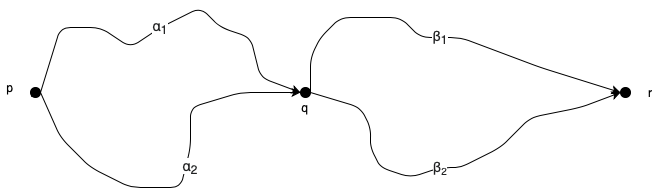
\includegraphics[scale = 0.5]{fotos_topo_2/otrasfotos/ex2.2.png}
\end{equation}
Anem a demostrar en primer lloc que la hipòtesi $\alpha_1\simeq \alpha_2$ és equivalent a $\overline{\alpha_2}*\alpha_1\simeq \varepsilon_q$, on $\varepsilon_q$ denota el camí constant en el punt $q$ i $\overline{\alpha}_2$ és el camí invers a $\alpha_2$, és a dir $\overline{\alpha}_2(t) = \alpha_2(1-t)$. Això es veu clar per la proposició (\ref{exercici2.1}), apartat (i), on es demostra que el producte està ben definit, ja que a partir d'això s'obté que si $\alpha_1\simeq\alpha_2$ aleshores $\overline{\alpha}_2*\alpha_1\simeq \overline{\alpha}_2*\alpha_2$ i això és trivialment homòtop al camí constant $\varepsilon_q$. Recíprocament, anem a demostrar que si $\overline{\alpha}_2*\alpha_1\simeq \varepsilon_q$ aleshores $\alpha_1\simeq \alpha_2$. Si $\overline{\alpha}_2*\alpha_1\simeq\varepsilon_q$, aleshores $\alpha_2*\overline{\alpha}_2*\alpha_1\simeq \alpha_2*\varepsilon_q\simeq\alpha_2$. D'altra banda, $\alpha_2*\overline{\alpha}_2*\alpha_1\simeq \varepsilon_q*\alpha_1\simeq\alpha_1$. Per tant obtenim $\alpha_1\simeq\alpha_2$ per la transitivitat de la relació d'homotopia de camins.

Ara, partim de la hipòtesi que $\alpha_1*\beta_1\simeq \alpha_2*\beta_2$ i fem $\overline{\alpha}_2*\alpha_1*\beta_1\simeq \overline{\alpha}_2*\alpha_2*\beta_2$, d'on $\varepsilon_q*\beta_1\simeq \varepsilon_q*\beta_2$ i, en definitiva $\beta_1\simeq\beta_2$.
\end{proof}






\end{document}